\begin{frame}{QAOA}{Quantum Approximate Optimisation Algorithm}
\begin{itemize}
    \item Given a cost function $f(x)$, define the \textit{problem Hamiltonian}:
\begin{align}
    \hat{H}_{P} \ket{\boldsymbol{x}} = f(\boldsymbol{x}) \ket{\boldsymbol{x}}. \label{eq:Hp}
\end{align} and another Hamiltonian called the \textit{mixer Hamiltonian} usually taken to be the transverse-field Hamiltonian:
\begin{align}
    \hat{H}_{m} = - \sum_{j} \hat{X}_{j}, \label{eq:Hm}
\end{align}
\item Define two parameterised unitaries: the \textit{phase operator}
    \begin{align}
        U_{P}(\gamma) = e^{-i \gamma \hat{H}_{P}} \label{eq:up}
    \end{align}
    and the \textit{Mixing operator:} \begin{align}
        U_{M}(\beta) = e^{-i \beta \hat{H}_{M}} \label{eq:um}
    \end{align}
\item Initial state: equal superposition $\ket{\psi_{i}} = \frac{1}{\sqrt{2^{n}}} \sum_{\boldsymbol{x}} \ket{\boldsymbol{x}}$
\end{itemize}
\end{frame}

\begin{frame}{QAOA}{circuit}
After $P$ alternating layers, the final state is
\begin{align}
    \ket{\boldsymbol\beta, \boldsymbol\gamma} &= \hat{U}_{M}(\beta_{P-1}) \hat{U}_{P}(\gamma_{P-1}) \cdots 
    \hat{U}_{M}(\beta_{0}) \hat{U}_{P}(\gamma_{0}) \ket{\psi_{i}}, \label{qaoa-equation}
\end{align}
\begin{figure}[H]
    \centering
    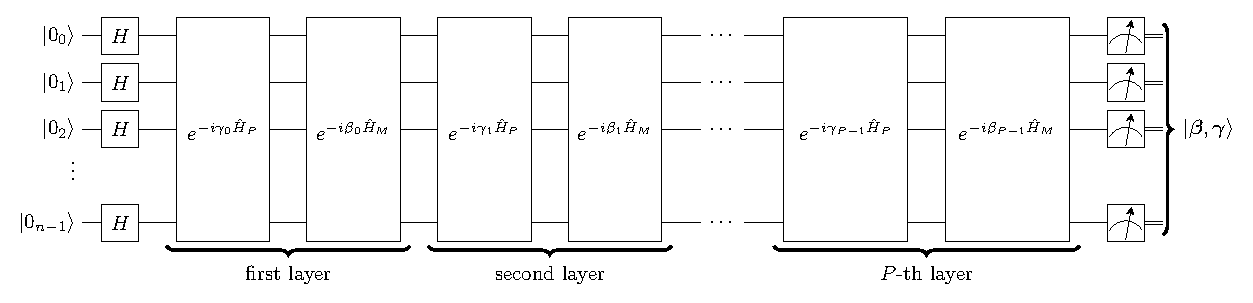
\includegraphics[width=\textwidth]{pictures/circdiagram.pdf}
    \caption{
        A $P$-layer QAOA circuit on $n$ qubits. Each layer applies a problem unitary 
    }
    \label{qaoa-circ}
\end{figure}
Objective: find parameters $(\boldsymbol{\beta}, \boldsymbol{\gamma})$ minimising
    \[
        \langle f \rangle = \bra{\boldsymbol\beta, \boldsymbol\gamma} H_{P} \ket{\boldsymbol\beta, \boldsymbol\gamma}.
    \]
\end{frame}

\begin{frame}{QAOA}{Quantum Alternating Operator Ansatz}
    \begin{itemize}
        \item Consider a problem where we only want to find a solution that belongs to a set of \textit{feasible} solution which is a (proper) subset of the set of all solutions.
        \item Using the tranverse-field Hamiltonian does not preserve the feasible subspace.
        \item The extension of the original QAOA introduced in \cite{Hadfield_2019-Quantum-Alternating-Operator-Ansatz-new-QAOA} allows the mixing Hamiltonian to be problem specific.
    \item Restricts dynamics to a feasible subspace $\Rightarrow$ guarantees valid solutions.
    \item Ensures all sampled solutions respect hard constraints.
    \end{itemize} 
\end{frame}
